%%%%%%%%%%%%%%%%%%%%%%%%%%%%
% Two Sword Lengths
% Christopher Gandrud
% 26 June 2013
%%%%%%%%%%%%%%%%%%%%%%%%%%%%

% !Rnw weave = knitr

\documentclass[a4paper]{article}\usepackage{graphicx, color}
%% maxwidth is the original width if it is less than linewidth
%% otherwise use linewidth (to make sure the graphics do not exceed the margin)
\makeatletter
\def\maxwidth{ %
  \ifdim\Gin@nat@width>\linewidth
    \linewidth
  \else
    \Gin@nat@width
  \fi
}
\makeatother

\definecolor{fgcolor}{rgb}{0.2, 0.2, 0.2}
\newcommand{\hlnumber}[1]{\textcolor[rgb]{0,0,0}{#1}}%
\newcommand{\hlfunctioncall}[1]{\textcolor[rgb]{0.501960784313725,0,0.329411764705882}{\textbf{#1}}}%
\newcommand{\hlstring}[1]{\textcolor[rgb]{0.6,0.6,1}{#1}}%
\newcommand{\hlkeyword}[1]{\textcolor[rgb]{0,0,0}{\textbf{#1}}}%
\newcommand{\hlargument}[1]{\textcolor[rgb]{0.690196078431373,0.250980392156863,0.0196078431372549}{#1}}%
\newcommand{\hlcomment}[1]{\textcolor[rgb]{0.180392156862745,0.6,0.341176470588235}{#1}}%
\newcommand{\hlroxygencomment}[1]{\textcolor[rgb]{0.43921568627451,0.47843137254902,0.701960784313725}{#1}}%
\newcommand{\hlformalargs}[1]{\textcolor[rgb]{0.690196078431373,0.250980392156863,0.0196078431372549}{#1}}%
\newcommand{\hleqformalargs}[1]{\textcolor[rgb]{0.690196078431373,0.250980392156863,0.0196078431372549}{#1}}%
\newcommand{\hlassignement}[1]{\textcolor[rgb]{0,0,0}{\textbf{#1}}}%
\newcommand{\hlpackage}[1]{\textcolor[rgb]{0.588235294117647,0.709803921568627,0.145098039215686}{#1}}%
\newcommand{\hlslot}[1]{\textit{#1}}%
\newcommand{\hlsymbol}[1]{\textcolor[rgb]{0,0,0}{#1}}%
\newcommand{\hlprompt}[1]{\textcolor[rgb]{0.2,0.2,0.2}{#1}}%

\usepackage{framed}
\makeatletter
\newenvironment{kframe}{%
 \def\at@end@of@kframe{}%
 \ifinner\ifhmode%
  \def\at@end@of@kframe{\end{minipage}}%
  \begin{minipage}{\columnwidth}%
 \fi\fi%
 \def\FrameCommand##1{\hskip\@totalleftmargin \hskip-\fboxsep
 \colorbox{shadecolor}{##1}\hskip-\fboxsep
     % There is no \\@totalrightmargin, so:
     \hskip-\linewidth \hskip-\@totalleftmargin \hskip\columnwidth}%
 \MakeFramed {\advance\hsize-\width
   \@totalleftmargin\z@ \linewidth\hsize
   \@setminipage}}%
 {\par\unskip\endMakeFramed%
 \at@end@of@kframe}
\makeatother

\definecolor{shadecolor}{rgb}{.97, .97, .97}
\definecolor{messagecolor}{rgb}{0, 0, 0}
\definecolor{warningcolor}{rgb}{1, 0, 1}
\definecolor{errorcolor}{rgb}{1, 0, 0}
\newenvironment{knitrout}{}{} % an empty environment to be redefined in TeX

\usepackage{alltt}
\usepackage{fullpage}
\usepackage{lscape}
\usepackage[authoryear]{natbib}
\usepackage{setspace}
    \doublespacing
\usepackage{hyperref}
\hypersetup{
    colorlinks,
    citecolor=black,
    filecolor=black,
    linkcolor=cyan,
    urlcolor=cyan
}
\usepackage{booktabs}
\usepackage{dcolumn}
\usepackage{url}
\usepackage{tikz}
\usepackage{todonotes}
\usepackage{verbatim}
\usepackage{endnotes}


\setlength{\belowcaptionskip}{0.5cm}

%%%%%%% Title Page %%%%%%%%%%%%%%%%%%%%%%%%%%%%%%%%%%%%%%%%%%%%
\title{Two Sword Lengths: Losers' Consent and Violence in National Legislatures}

\author{Christopher Gandrud\thanks{Lecture in International Relations at Yonsei University (\href{mailto:gandrud@yonsei.ac.kr}{gandrud@yonsei.ac.kr}). Thank you to Simon Hix for very helpful comments, Hortense Badarani for research assistance, seminar participants at Yonsei University, and my GV101 students at the LSE for inspiration.
}}
\date{}
\IfFileExists{upquote.sty}{\usepackage{upquote}}{}

\begin{document}

\maketitle

%%%%%%% Abstract %%%%%%%%%%%%%%%%%%%%%%%%%%%%%%%%%%%%%%%%%%%%
\begin{abstract}
National legislative chambers should be venues for peacefully resolving conflicts between opposing groups. However, they can sometimes become the scenes of physical violence between legislators. Legislative violence is an indication that a country's democratic institutions are functioning far from perfectly as legislative losers are deciding to drop out of the `game', rather than consent to the winners' decisions. In order to better understand these situations I use a new data set to examine what features are associated with violence in national legislative chambers. My main findings are that established democracies, democracies with highly proportional electoral outcomes and with large governing majorities are less likely to have legislative brawls.

\end{abstract}


\paragraph{Keywords:} legislatures, violence, electoral proportionality, institutional design, democratic consolidation, losers' consent

\vspace{0.3cm}

%%%%%%% Introduction %%%%%%%%%%%%%%%%%%%%%%%%%%%%%%%%%%%%%%%%%%%%

Though legislators are often described as `battling' or `fighting' we generally expect these battles to be in terms of rhetoric and procedural maneuvers culminating in votes. The outcomes of these contests are then respected by all legislators, even those on the losing side. Unfortunately, metaphorical battles sometimes become physical fights between members of legislatures. 

Thankfully rare, physical conflicts nonetheless have a history of breaking out in lawmaking chambers between members. The history of many legislative chambers contains incidences of violence. In 1856 Preston Brooks, a member of the United States House of Representatives, canned Senator Charles Sumner unconscious in the Senate chamber in a dispute over slavery \citep{USSenateCanning}. It has even been suggested that the United Kingdom's House of Commons is physically designed to prevent violence between members. The Government and Opposition benches are said to be ``two sword lengths apart" \citep{ParliamentUKSword} so that duels will be fought with words rather than swords. Actual, sword fights do not seem to have taken place in the Commons chamber, but violent incidences did occur. For example, in 1893 a fight broke out between Irish nationalist and Unionist members of parliament \citep{ByrneViolence}. Violence in legislatures continues to occur, with incidences being regularly reported on by the media.\endnote{The Guardian newspaper, for example, sporadically compiles stories of physical fights in legislative chambers. See \url{http://www.guardian.co.uk/politics/gallery/2010/dec/17/1\#/?picture=369861052\&index=0}. Legislative violence has also has its own Wikipedia page. See {\url{http://en.wikipedia.org/wiki/Legislative_violence}}.} Recent incidences of violence between legislators include multiple brawls in Ukraine in 2010 and in South Korea in 2009. In both instances opposition legislators, facing impending legislative defeats, tried to obstruct the governments' attempts to pass controversial legislation.\endnote{In Ukraine the fight was over Russian military bases and in South Korea it concerned media ownership laws.} 

Contestation is an important part of democracy \citep{Alvarez1996, Dahl1971, Follesdal2006}, but extreme contestation in the form of legislative violence indicates a dysfunctional democracy. Contestation creates winners and losers and democracy in particular ``is a system in which parties lose elections" \citep[][10]{Przeworski1991}.  In well functioning democracies losers accept the legitimacy of the contest's rules \citep[][553]{Nadeau1993} and consent to follow the winners' decisions \citep[][]{Anderson2005}. Legislative losers\endnote{I define {\emph{legislative losers}} as actors who are unable to use legislative procedures to at least block policy changes that they prefer less than the status quo. {\emph{Winners}} are actors that can use legislative procedures to at least block a change that they prefer less than the status quo. The winner concept is the same as a ``veto player" \citep[see][]{Tsebelis2002}.} who use violence are not consenting to decisions made by the winners. At least some legislators do not believe that voting and other parliamentary procedures, or at least the current implementation of the procedures is legitimate. They are not `playing by the rules of the game', but instead taking extreme extra-procedural actions to influence outcomes. 

Such choices have troubling implications for the quality and long-term prospects of democracy. \citeauthor{Anderson2005} argue that ``the consent of the losers is one of the central, if not {\emph{the}} central requirements of the democratic bargain" that determines who can authoritatively allocate values in a given society \citeyearpar[][2-4]{Anderson2005}. Legislative violence indicates that some people on the losing side are deciding to stop playing by democratic rules and are instead choosing paths other than than democracy to achieve their goals. Furthermore, legislative violence may undermine citizens' satisfaction with democracy and threaten processes of democratic consolidation in new democracies. Public ``appreciation" of the legislature is part of a strong political society, which is a key component of democratic consolidation \citep{Stepan1996}. The violent spectacles that legislative brawls often become may hurt this appreciation and ultimately the public's satisfaction with democracy. 

\begin{center}

    {\bf{[Figure 1 About Here]}}

\end{center}

Despite their history and negative implications for the quality of democracy, incidences of legislative violence have largely been ignored by academic political scientists. To systematically study legislative violence I used the Google News Archive\endnote{See {\url{http://news.google.com/archivesearch}}.} to create a data set of {\emph{physical fights between legislators in national legislative chambers}}.\endnote{The Google News Archive search was conducted in Spring 2011. Please contact me for a complete list of sources and search terms.} This resulted in a data set of 88 incidences of legislative violence in 30 countries between 1981 and Winter 2011. We can see in Figure \ref{leg_map} that these events have occurred in many countries around the world. They do not apear to be confined to any one cultural group or region. Violence is nonetheless not evenly distributed across countries. I observed 30 countries having incidences of legislative violence, but over 60 percent of these fights occurred in eight countries with four or more total legislative brawls. Legislative violence appears to be found more often in weaker and newer democracies like Ukraine's, Mexico's, South Korea's and Taiwan's. This association is illustrated in Figure \ref{UDSAgeScatter}. The figure simply plots countries' Unified Democracy Scores (UDS) \citep{Pemstein2010}\endnote{The scores were found through Bayesian latent variable analysis using 10 measures of democracy, including Freedom House, Polity, and so on. I only use posterior mean UDS scores in this paper. See \cite{Pemstein2010} for a discussion of UDS' advantages over individual measures of democracy. Though there is no direct substantive meaning to individual values, higher positive values can be thought of as indicating more democracy.} in a given year against how many years they had Polity scores greater than 5.\endnote{Five is the qualitative point the creators of the data set choose for determining if a country is democratic or not \citep{Marshall2009}. I did not use UDS to determine democratic age because, unlike the Polity measure, UDS scores do not have a clear substantively meaningful cutoff point which we can use to code a country as being democratic or not.} Parliaments with violence are predominantly in weaker democracies with mean UDS scores ranging mostly from just below 0 to about 1.5. Legislative violence is not observed in any country with a democracy over 60 years old.

\begin{center}

    {\bf{[Figure 2 About Here]}}

\end{center}


This brief tour of descriptive statistics suggests that violence between legislators does not occur randomly. Instead violence appears to be a characteristic of new and and weak democracies. There is a considerable literature on how the age of a democratic regime and its type of institutions can affect citizens' satisfaction and support for democracy \citep{Aarts2008, lijphart1999, Norris1999, Wagner2009}--particularly citizens on the losing side \citep{Anderson1997, Anderson2001, Anderson2005, Bernauer2011, Blais2007}. Most of the literature on losers' has examined why voters may or may not become dissatisfied when the candidate or party they voted for does not win an election. Legislative violence is an indicator of another important group's--legislative losers--(dis)satisfaction with democracy. 

Building on research into why losers consent to follow the decisions of lawmaking winners and Arend Lijphart's related work on majoritarian and consensual democratic designs \citeyearpar{Lijphart1977, Lijphart1984, Lijphart1991, lijphart1999, Lijphart2003, Lijphart2004}, I develop a framework for understanding when violence in national legislatures is more or less likely. {\emph{Violence is more likely when there are larger gaps between winners and losers.}}\endnote{The `winner-loser gap' concept is from Anderson et al. \citeyearpar[10]{Anderson2005}. See also \cite{Blais2007}.} Bigger gaps make losing more painful and consenting to winners' decisions more difficult. For legislative violence the key gaps are between winners' and losers' {\emph{experience}} in both roles under the current rules of the game, gaps in {\emph{representation}}--i.e. electoral disporoportionality--, as well as a combined {\emph{preference}} and lawmaking \emph{power} gap, or the gap in the degree to which winners are able to move policies to their ideal preferences and away from losers'.\endnote{\cite{Anderson2005} and \cite{Blais2007} were generally more concerned with citizens, than decision-makers so they focused on gaps of experience and preference. Since I am concerned with legislative decision-makers, I expand the concept to also include representation and power gaps.} 

Experience gaps tend to be a function of democratic age since the older a democracy is the more likely it is that present winners and losers have had experience in the other position. New democracies may also have wider gaps in preferences and possibly power. Gaps in representation are largely a function of the electoral system. Proportional electoral systems tend to produce smaller gaps between winners' and losers' vote shares and seat shares. Majoritarian electoral systems tend to create bigger gaps. Preference and power gaps can be shaped by lawmaking institutions, with majoritarian systems usually producing bigger gaps than consensual ones. From this framework I expect that newer democracies are more likely to have violence and that this tendency will be stronger under majoritarian arrangements. Testing this approach will hopefully aid our understanding of how lawmaking institutions could be designed to improve the likelihood that legislative losers will continue playing by the rules of the democratic game.

In this paper I first use the losers' consent and consensual institutions literatures to develop my framework for understanding the conditions under which legislative violence is more likely. I then briefly discuss other political science approaches that may provide competing alternative explanations of legislative violence. In particular I discuss how Inglehart and Welzel's \citep{Inglehart1988, Inglehart2005, Inglehart2010} seminal work on values and democratization provides a competing set of explanations. After discussing previous research, I begin an empirical investigation of my framework and the alternative explanations by discussing the variables and rare event logistic regression models \citep{KingRareEvents2001, KingRareEventsPA2001} I use to study these (thankfully) rare events. Finally, I lay out my findings that established democracies, democracies with highly proportional legislatures and large governing majorities are less likely to have legislative brawls. These results suggest that violence between legislators is less likely when the gaps between winners' and losers' experience, representation, preferences and power are smaller.

%%%%%%%%%%%%%%%%%%%%%%%%%%%%%%%%%%%%%%%%%%%%%% Previous Research & Framework

\section{Previous Research on Losers' Consent \& Its Predictions for Legislative Violence}

\cite{Anderson2005} highlight two broad factors that influence the gaps between winners and losers. These gaps may affect the probability that losers will consent and continue playing by the rules of the game. First, they argue that winner-loser gaps tend to be larger in new democracies. Second, building on Lijphart's discussion of majoritarian and consensual democratic institutions, they argue that some institutions, irrespective of democratic age, can exacerbate or mitigate the strength of winners' wins and losers' losses.

\subsection{Losers in New vs. Old Democracies}

We have already seen how legislative violence is almost non-existent in older democracies, i.e. losers in older democracies almost always consent to lawmaking winners' decisions, at least to the extent that they do not use violence in legislative chambers. Speaking generally about support for democracy, Anderson et al. \citeyearpar[Chapter 6]{Anderson2005} give a number of reasons for why it is harder for losers to consent in new compared to old democracies. 

Even under the best circumstances, losing can be more painful and may produce higher dissatisfaction in new compared to old democracies. The gaps between winners' and losers' experiences in the other position tend to be much larger in new democracies. This is illustrated in the top pair of lines in Figure \ref{example_gaps}. In new democracies actors simply have not had the time to learn that they can someday become winners. Losers in new democracies may not have learned that ``pretenders to office can expect to reach it, losers can expect to come back" \citep[][36]{Przeworski1991}.

Furthermore, in new democracies the rules of the game are in flux. This can give present winners considerable power. Incumbent actors may be better able to establish rules that entrench their power before the democratic regime has fully consolidated. Not being involved in institutional rulemaking could have major long-term implications for losers as the rules that are established may fix them as losers for many years to come. If this is the case, losers would develop a belief that they will not be able to experience being winners in the future. They may believe that the gaping experience gap is going to persist. They would therefore have less incentive to continue playing by the rules of the game. 

Another general feature of new democracies is a large winner-loser preference gap. In new democracies ``outputs produced by different political camps are likely to constitute more divergent visions of the good society than in more established [democracies]" \citep[][92]{Anderson2005}. New policies tend to be farther away from losers' preferences and are therefore harder to accept. I discuss this type of gap in more detail below.

If losers are unable to become winners, we may not expect to see the new democracy become an old one. \citeauthor{Przeworski1991} describes successful democratic institutions as ones ``that reduce the stakes of political battles" \citeyearpar[][36]{Przeworski1991}. Institutions that entrench aggrieved losers do the opposite. They heighten political battles by potentially making each new law an irrevocable--or at least highly sticky--change to the status quo in a direction less preferred by the losers. If these processes lead to democratic collapse, such countries would simply not be included in any sample for us to observe them having incidences of legislative violence as old democracies. 

\begin{center}

    {\bf{[Figure 3 About Here]}}

\end{center}


\subsection{Consensual Institutions \& Losing}

Some institutions may be able to decrease the gaps between winners and losers more effectively than others. Anderson et al. \citeyearpar[Chapter 7]{Anderson2005} largely draw on Lijphart's literature of consensual democratic institutions \citeyearpar{Lijphart1977, Lijphart1984, Lijphart1991, lijphart1999, Lijphart2004} to understand how institutions shape winner-loser gaps.\endnote{See also \cite{Bernauer2011} for an examination of how consensual institutions, particularly consensual cabinets and direct democracy improve citizen-level losers' satisfaction with democracy.} As the ``rules of the game" \citep{North1990} institutions are in essence the structures by which losers are created. Consensual institutions such as electoral systems that produce proportional outcomes, coalition governments and federalism may help  minimize the gaps in winners' and losers' electoral representation, preferences and power in decision-making bodies. Majoritarian institutions such as electoral systems that create disproportional outcomes and single party governments could exacerbate these gaps.

Proportional electoral systems are important institutions for determining winner-loser representation gaps.\endnote{\cite{Lijphart2004} refers to electoral system design as ``the most important choice" for a democracy to make. See also \cite{Diamond1999}.} Proportional electoral systems are associated with more consensual types of democracy \citep{Powell2000} as they create fewer unrepresented segments of society. Proportional outcomes create legislatures that are a ``microcosm of society" \citep{Carey2011}. For studying legislative violence we are more interested in the fact that proportional outcomes minimize the gap between how winners and losers are represented in the legislature. Disproportional outcomes, like those created by first-past-the-post electoral systems \citep[see][]{Duverger1954}, exacerbate representational gaps. 

Figure \ref{example_gaps}.B illustrates the representational gaps between winners and losers when there are disproportional compared to more proportional electoral outcomes.  The difference in the ratios of winning parties' and losing parties' seats to votes shares\endnote{If the ratio equals one then the proportion of seats that a party wins is equal to its proportion of votes.} is much smaller when there are proportional rather than disproportional outcomes. Losers may be more likely to view legislative outcomes as illegitimate if they are created by winners whose representation is much larger than their vote shares. Consenting to these outcomes could be harder.

The exact type of electoral system is interesting to us from an institutional design point of view, but we should not confuse ``the outcome of an electoral system with its mechanics" \citep[][109]{Golder2005}.\endnote{How proportional an outcome is can be affected by both electoral system rules and the distribution of party support within a country, for example.} When studying how elections influence the propensity of losers to use legislative violence we are more interested in how proportional electoral outcomes are, rather than the exact type of electoral system that produced these outcomes. 

Along with proportional electoral outcomes, which tend to increase the diversity of actors in a parliament, other institutions can influence preference gaps and the boundaries of winners' power by altering the number and type of veto players that can stop policy change \citep{Tsebelis2002}. Consensual institutions tend to increase the number of veto players, whereas majoritarian institutions have the opposite effect. As the number of veto players increases it becomes harder to change the status quo policy.\endnote{To use Tsebelis' terminology, the winset--the set of policy changes that could be accepted by the veto players--decreases or at least stays the same as the number of veto players increases \citeyearpar[][24]{Tsebelis2002}.} As the number of veto players increases there are also more opportunities for these actors to have dissimilar preferences, possibly shrinking the winner-loser preference gap. The result of combined large power and preference gaps is that losers can be made much worse off by policy changes. These changes will be harder to consent to. Legislators may therefore be more likely to use violence.

The relationship between preferences, power and winner loser gaps is illustrated in Figure \ref{example_gaps}.C. In the majoritarian example the right most actor is the winner. The status quo policy is at the left most actor's ideal point. Because the right most actor is the only winner, it is very powerful and can move the policy very close to its ideal point. Because its ideal preference is very far from the losers', the loser is much worse off than they were before. Conversely, in the consensual example there are two winners ($W_{1}$ and $W_{2}$). Though $W_{2}$ has the same ideal point as the winner in the previous example, they have less power because they need the agreement of $W_{1}$ to move policy closer to their ideal point. If the status quo is at the loser's ideal point then the new policy will move to $W_{1}$'s ideal point. $W_{1}$ most prefers this point and $W_{2}$ prefers it more than the status quo.\endnote{These examples assume equal agenda setting power. Even if $W_{2}$ was the sole agenda setter the new policy would be closer to $L$'s preferences--the winner-loser gap would be smaller--in the consensual compared to the majoritarian example.} This outcome is much more preferable for the loser than the outcome in the majoritarian  scenario.

Executive regime type could be important for shaping the power/preference gap. Linz \citeyearpar{LinzPres1990, LinzParl1990} argues that parliamentary systems allow for the creation of flexible coalitions between multiple parties. In multiparty coalitions there is a greater probability that the gaps between winners and losers will be smaller. Coalitions possibly include a wider variety of preferences than single party governments. Parliamentary coalitions also forestall the creation of zero-sum games, which produce severe losses. No one party takes all of the lawmaking power. Parties not currently in power may also reasonably expect to be a coalition partner in the future and have an incentive to continue playing by standard legislative rules. Linz particularly argues that coalition parliamentary systems are superior to presidential ones. In presidential systems there is clearly only one president and so elections are largely `winner-takes-all'. This creates zero-sum games with severe losses. 

It is important to note that a number of authors, chiefly \cite{Horowitz1990}, believe that Linz inaccurately characterizes presidential systems. Depending on how power is officially divided between the president and parliament and especially if the two are controlled by different parties, presidential systems may be as consensual as coalition parliaments.

Federalism is another consensus-type institution that may be able to mitigate the severity of losers' losses. National-level losers may still be able to share in decision-making if they are able to gain power in geographically more concentrated provincial-level elections \citep{Anderson2005, Lijphart2004}. Though not directly related to national legislative politics, perhaps national legislators on the losing side will continue to play the game because their interests can be advanced at lower levels of government. 

The consensus approach to institutional loss mitigation suggests that electoral systems producing proportional outcomes, parliamentary coalition government and a federal distribution of power minimize disproportional representation and the preference and power gaps between winners and losers. 

\vspace{0.5cm}

\subsection{A Framework for Predicting Legislative Violence}

From this discussion I develop a framework for predicting when legislative violence is more likely. The framework is summarized in Table \ref{leg.v.framework}. The two key dimensions of the framework are {\emph{age of democracy}} and whether or not there is a  {\emph{consensual}} system. South Korea is an example of a `perfect storm' country with both a new democracy and has a fairly majoritarian system. It became a democracy within the past 20 years, its mixed legislative electoral system produces relatively disproportional outcomes,\endnote{South Korea's average disproportionality as measured by the Gallagher Index \citep[][see the discussion below for further details]{Gallagher1991, Gallagher2012} from 2000 until 2011 was 12.7. This places it in the upper 25 percent of observations with democratic legislatures.} it has a presidential system where the president is even involved in appointing the leader of the legislature--the prime minister--and it has a largely centralized geographical distribution of power.\endnote{Though provincial and local governments are elected, deputy executives who have detailed administrative powers are appointed by the central government.} South Korea had eight observed incidence of legislative violence in my sample.

I assume a best case framework in that a lack of a consensual system or an established democracy could be compensated for by the existence of the other characteristic. For example, new democracies could compensate for a lack of experience with democracy by having highly consensual instititutions. South Africa is an example of this type of country. Though there has not been an alternation of the party in power--the African National Congress--since it became a democracy in the mid-1990s, South Africa has very proportional electoral outcomes,\endnote{South Africa's average Gallagher disproportionality was 0.29 from 2000 until 2011, one of the lowest observed in the sample.} a parliamentary system usually governed by a generally inclusive super-majority party\endnote{More inclusive parties may be similar to multiparty coalition in that they have a wide range of preferences thereby decreasing the winner-loser preference gap.} and federalism. I did not observe it having an incident of electoral violence. Old democracies with generally unfair distributions of power should be less likely to have violence because over time legislators learn to be both winners and losers. The United Kingdom is an example of this. Its plurality electoral system generally produces disproportional outcomes,\endnote{It had an average disproportionality of 16.5 from 2000 to 2011} but both left-leaning Labour and right-leaning Conservative parties have had experience in government, can expect to be in government in the future, even if they are currently in opposition, and will have an opportunity to be able to change policies enacted when they were in opposition that they greatly dislike. Finally, countries with both old democracies and fair distributions of power are clearly unlikely to have legislative violence according to this framework. Sweden is a good example of such a country. 

\begin{center}

    {\bf{[Table 1 About Here]}}

\end{center} 

\section{Alternative Explanations}

Of course there may be other factors inclining legislators towards violence. I briefly discuss two of these possible alternative explanations: culture and hard rules prohibiting violence.

\subsection{Trusting Cultures}

Ingelhart and Welzel \citep{Inglehart1988, Inglehart2005, Inglehart2010} have been the main contemporary proponents of a link between cultural values and democracy. Using their World Values Survey Data \citeyearpar[the most recent version is from][]{WVS2009}, they find that ``self-expressive values" are both enduring cultural traits and positively associated with democratic stability. They include in this category participation, life satisfaction, norms of cooperation and trust.\endnote{\cite{Tyler1998} makes a distinction between trust in others and trust in authority. The former is much more conducive to democracy than the latter.} 

The same processes that might be behind self-expression and democratic stability might also lead to less legislative violence. Life dissatisfaction could heighten tensions between legislators, especially legislators that are out of and in power. A lack of trust and sense of reciprocity might incline legislative losers to not believe that legislative rules are being followed by the opposing side \citep{Tyler1998}, making their losses more severe. These beliefs could make violence seem like a more meaningful way of influencing policy than playing by the rules. According to this approach some legislatures have less trusting members who would therefore view a loss in a much more negative light and be less likely to believe that they will someday become winners under the current rules of the game. As a result losers in less trusting societies could be more likely to resort to violence. 

We saw earlier that legislative violence has not been confined to one cultural region, nonetheless some have argued that specific regional cultures are less likely to respect democratic institutions. These cultures might be more likely to have legislative violence. The many popular hypotheses about East Asian cultures\endnote{These are often referred to as `Confusion' cultures \citep{Inglehart2005, Inglehart2010}.} and democratic instability are especially relevant for us given the high number of brawls in East Asia, notably in Japan, South Korea and Taiwan (see Figure \ref{leg_map}). One view is that Asian societies have hierarchical and deferential cultures that are incompatible with democracy because authority is valued over self-expression \citep[see][212-213 for a discussion]{Dalton2005}. It is unclear how this hypothesis would explain the high frequency of legislative violence in Asian democracies. It would seem to actually suggest less violence. Recent empirical evidence has suggested that Asian societies are in fact not strongly deferential to authority, especially when compared to Western ones \citep{Dalton2005, KimAsianValues2010}. Mostly using Inglehart and Welzel's World Values Survey data, \cite{KimAsianValues2010} actually finds that East Asian societies have lower respect for authority than non-Asians and Southeast Asians. Assuming that societal values are generally congruent with legislators' values, perhaps legislators in East Asian countries are more violent because their members do not respect and trust legislative authorities. Legislative violence in this region would thus simply be the result of the same proximate cause as in any other low-trust society. As such, examining the effect of trust should capture any `East Asian cultural' effect. 

This and any piece of research examining the effect of institutions on political conflict face an endogeneity problem when trying to determine how institutions are related to conflict \citep[][751]{Carey2000}. There is an old tradition in political science \citep[][528--529]{Frye1997} arguing that culture influences institutional choice \citep[in particular see][]{Almond1963}. For example, certain cultures may be more consensual and are therefore likely to adopt consensus institutions \citep[][22-23]{Lijphart2003}. Relationships between institutions and violence could be spurious. Consensual societies may choose certain institutions and also be less violent in general, resulting in less violence between legislators. Consensual institutions may then reinforce consensual cultures and so on. These are not issues I solve here. Instead we should at least be mindful of them especially when drawing conclusions from the following analysis.

\subsection{Legislative Immunity \& Violence}

Finally, beyond the fairness of the distribution of legislative power there is another institutional design feature that might prevent violence. Like in society generally, having laws that outlaw violence and sanction violators of these laws may dissuade physical attacks. In many countries legislators are immune from prosecution or at least arrest in the legislative chamber. Such immunity is often granted in order to prevent the legislature from being harassed and obstructed by the executive or judicial branches of government  \citep{Seghetti1984}. However, legislators immune from legal consequences may be more likely to physically harass and obstruct one another in order to prevent or put off losing. Legislators who do not have this immunity might be less likely to attack their colleagues.

%%%%%%%%%%%%%%%%%%%%%%%%%%%%%%%%%%%%%%%%%%%%%%%%%%%%%%%%%%%%%%%%%%%%%%%%%%% Empirical Analysis
\section{Empirical Analysis: What is Associated with Legislative Brawls?}

To empirically examine the associations between age of democracy, institutions, culture and legislative violence I use incidences of legislative brawls as the dependent variable in a series of rare events logistic regression models \citep{KingRareEvents2001, KingRareEventsPA2001}. I use a number of familiar variables and data sources to operationalize institutional and societal concepts discussed in the literature review. A matrix illustrating the variables' correlations can be found in Figure \ref{corrmatrix} in the Appendix. This figure also includes the variables' observed minimum and maximum values for reference. Variable descriptions and sources are summarized in Table \ref{var_summary}, also in the Appendix. Following Gary King's \citeyearpar{King1995} recommendation, full replication data and code used for all of the analyses can be found in this document's markup file and accompanying {\tt{R}} files.\endnote{The main data file is in Stata format and can be found at: {\url{https://www.dropbox.com/s/9kn73p98bb7lynh/leg_violence_main.dta}}. \\ Markup files can be found at {\url{https://www.dropbox.com/sh/vuu9si2188255sw/AoxQL19Z9k}}.}

%%%%%%%%%%%%%%%%%%%%%%%%%%%%%%%%%%%%%%%%%%%% Independent variables
\subsection{Right-hand Variables}

We already saw a possible association between the age of democracy and incidences of violence. As mentioned earlier, I measure the {\emph{age of a democratic regime}} as the number of years a country's Polity score is greater than five.

Older democracies are more likely to have higher proportions of legislators who have actually experienced being both winners and losers. I would have liked to more directly model the effects of legislator tenure by including some measures of the time legislators are in office. Unfortunately, I was unable to find data on legislator tenure for the range of countries included in the sample. As a proxy I include the {\emph{tenure of the shortest serving veto player}} variable from the Database of Political Institutions (DPI) \citep[updated to 2010]{DPI2001}. In this data set veto players are either the prime minister and major parliamentary parties or the president and the largest legislative party.

I occasionally include Unified Democracy Scores (discussed earlier) as a measure of democratic quality. Generally in the analyses below UDS is negatively associated with violence. However, since I am more concerned about what particular aspects of democracy are associated with violence I do not discuss these results in detail.

I use two variables to examine the relationship between the fairness of electoral outcomes and violence. The first is simply a dummy of whether or not a country's legislature is elected by some form of {\emph{proportional electoral system}}. The variable is from the DPI database. As noted earlier, simply looking at the electoral mechanics confuses mechanisms with outcomes. So, more importantly, I use the standard Least Squares or Gallagher Index \citep[see][]{Gallagher1991} to measure realized {\emph{electoral disproportionality}}.\endnote{Carey and Hix refer to the Index as the ``established means of measuring proportionality in electoral systems" \citeyearpar[387]{Carey2011}. The index is calculated for each election with the following equation: $ \mathrm{LS} = \sqrt{\frac{1}{2}\displaystyle\sum_{i=1}^{n} (v_{i}-S_{i})^2}$, where $V_i$ is the vote share for party $i$ and $S_{i}$ is party $i$'s seat share.} To gain maximum coverage, I compiled the data from both \cite{Gallagher2012} and \cite{Carey2011}.\endnote{Full details can be found at {\url{http://christophergandrud.github.com/Disproportionality_Data/}}.} A country's disproportionality score is treated as constant from the year of an election until the year before the following election. Higher values on the Gallagher Index indicate more disproportional, i.e. less fair electoral outcomes.

The consensus literature posits a number of other factors that may be important for shaping the proportion of losers and the severity of their loss. I include various measures of the distribution of lawmaking power in an attempt to account for these factors. I use the government {\emph{system}}--presidential, parliamentary, or mixed assembly-elected presidential--variable from DPI. To get a sense of the proportion of legislative losers I include a government {\emph{majority}} variable (from DPI) that simply measures the seats held by governing parties as a proportion of all seats. I transformed the variable from a proportion to a percentage to ease interpretation. Larger majorities would indicate that there are possibly more legislative veto players with more divergent preferences. To directly assess the effect of coalition compared to single-party governments I included the DPI {\emph{government fractionalization}} variable. It is the probability that two randomly picked deputies in the government are from different parties. I used the fractionalization variable to create an indicator of {\emph{single-party}} government. It is simply a dummy equaling one if fractionalization was zero, i.e. all governing legislators were from the same party. In general single party governments probably are better able to pass policies very close to their ideal preferences. This could heighten losers' loss.

I also include standard measures of the \emph{effective number of parliamentary parties} by votes and by seats \citep[see][]{Laakso1979, Taagepera1989}. The data was taken from \cite{Carey2011}\endnote{Their data is mostly from \cite{Golder2005}. Please see their notes for further details.} before 2004 and from \cite{Gallagher2012} afterwards. Both of these measures indicate how fragmented a parliamentary party system is. Higher scores indicate that there are more parties that win either votes or seats.

To examine whether or not national legislative losers may be dissuaded from legislative violence because there is a possibility of gaining power at a provincial-level, I include the \emph{federalism} dummy variable from \cite{Carey2011}.\endnote{Their data is mostly from \cite{Adsera2003}. Please see their notes for further details.} I updated this from 2004 until the end of the observation period.

In general Gallagher disproportionality scores will be the most direct way of operationalizing a winner-loser gap. They directly capture the winner-loser representation gap. The power/preference gap is very hard to operationalize across the range of countries included in this analysis. Indicators such as parliamentary or presidential government \citep{Horowitz1990}, electoral systems \cite{Lijphart1994}, the size of the governments' majority and federalism are poor approximations of this gap. In many cases there are considerable interactions between these factors, parliamentary rules and the distribution of a interests across a country that can greatly impact the power/preference gap. For example, presidential systems that give relatively equal power to both the president and legislature could be much more consensual than a single party majority parliamentary system if the president and legislature are controlled by different parties. I attempt to capture these sorts of interactions in the analysis, but this is empirically difficult. Given the small number of actual observed incidences of legislative violence there simply might not be enough information in the data to draw meaningful conclusions about these types of relationship \citep[see][]{Brambor2006}.

Legislators may be less likely to attack one another if they know that they could be arrested for assault. To examine this possibility I include Fish and Koening's \citeyearpar{Fish2009} dichotomous \emph{legislator immunity} variable. It equals one if national legislators are immune from arrest and/or prosecution and zero otherwise. Unfortunately, their data only captures legislative immunity in 2007. I extrapolated the 2007 value of the variable to the other observation years.\endnote{I also considered using the legislator immunity variable from the Comparative Constitutions Project \citep{ElkinsCCP2010}. However, the coding of the immunity variable is vaguer than Fish and Koening's and only deals with constitutionally mandated immunity.} We should therefore approach results from this variable with some caution since it might not be a valid indicator for all country-year observations.

To examine the relationships between societal-level values and legislative violence I rely primarily on data from the World Values Survey \citep{WVS2009}. Over the course of his research, Ingelhart has found that his composite {\emph{self-expression}} indicator was the best way to capture cultural and normative differences between democracies and non-democracies. Societies have high self-expression scores if they emphasize ``liberty and participation, public self-expression, tolerance of diversity, interpersonal trust, and life satisfaction" \citep[64]{Inglehart2003}. I focus on both the self-expression variable and the component {\emph{trust}} variable\endnote{Higher values on the trust variable indicate less trust.} from World Values Survey because it makes the most intuitive sense that legislators from societies that are very trusting may be less likely to resort to violence in the legislative chamber. Following \cite{Inglehart2003} I average the variables across individual participants within countries and survey waves. I only use the third through fifth survey waves\endnote{The surveys were taken in the following years: \\ Wave 3: 1994--1998 \\ Wave 4: 1999--2004 \\ Wave 5: 2005--2007} as the first two waves have very poor coverage. I used wave 3 for all years before 1998, wave 4 for all years between 1999 and 2004 and wave 5 onward. 

I include a number of other societal-level variables to help defend against omitted variable bias. Conflict in more ethnically or economically divided societies may be generally more intense. These conflicts may spill over into legislatures where they precipitate violence between members. I include Alesina et al.'s \citeyearpar{Alesina2003} {\emph{ethnic fractionalization}} data to account for the fact that a legislature's composition in terms of its fractionalization is not only a function of political institutions, but also social divisions \citep{Neto1997, Mozaffar2003}. The variable measures the probability that two randomly selected members of society will be from different ethnic groups. Higher values indicate more societal fractionalization. To capture similar possible effects of economic divisions, I include {\emph{Gini coefficients of economic inequality}} from \cite{UNU2008}.\endnote{Note, for country-years with missing data I assumed that the Gini Coefficient remained constant from the last year there is data for the country, unless the span was ten years or more. If this was the case they were treated as missing.} Finally, as is common in cross-country analyses, I also include {\emph{gross domestic product per capita}} in some of the models. This data is from the World Bank's International Development Indicators \citeyearpar{WorldBank2011} and is in thousands of United States dollars.

%%%%%%%%%%%%%%%%%%%%%%%%%%%%%%%%%%%%%%%%%%%% Empirical Model
\subsection{The Empirical Model: Rare Logistic Regression}

Thankfully, legislative brawls are rare. The overwhelming majority of legislatures, most of the time do not break out into physical fights. However, the rarity of legislative brawls creates some empirical problems. Standard logistic regression techniques can ``sharply underestimate the probability of rare events" and ``commonly used data collection strategies are grossly inefficient for rare events data" \cite[137]{KingRareEventsPA2001}. In this project the second problem is not too large. Using the methods described in the introduction, I focused on gathering information on as many legislative brawls in the past thirty years as possible. Unlike country-dyads for the study of war, for example, non-legislative violence data in the form of country-years\endnote{Legislatures with multiple incidences of violence in a single year have multiple observations for that year.} over the same time period was relatively not too difficult to collect. Data collection resulted in a very manageably sized data set with thousands of observations.\endnote{I assume that if no brawl was observe using the data gathering procedures discussed above that no violence occurred.} The first issue nonetheless presented a problem.

We are interested in a dichotomous outcome $Y_{i}\; (i = 1, \ldots, n)$: a legislature had an brawl $(Y_{i} = 1)$ or it did not $(Y_{i} = 0)$. Logit analysis is a standard way of estimating the effect of some covariates $\mathbf{x}_{i}$ on our main quantity of interest, the probability $\pi_{i}$ of observing $Y_{i} = 1$.\endnote{The probability of $(Y_{i} = 0)$ is $1 - \pi_{i}$} It consists of a stocastic component
%
\begin{equation}
    Y_{i} \sim \mathrm{Bernoulli}(\pi_{i})
\end{equation}
%
and a systematic component 
%
\begin{equation}
    \pi_{i} = \frac{1}{1 + \mathrm{exp}(-\mathbf{x}_{i} \beta)},
\end{equation}
%
where $\mathrm{\beta}$ are the coefficients.

\cite{KingRareEventsPA2001} demonstrate that in logit analysis with relatively very fewer observed events than nonevents--many more 0s than 1s--estimated coefficients $\mathbf{\hat\beta}$ will be too small. Furthermore, standard methods for computing event probabilities with logistic regression produce results biased in the same direction as $\mathbf{\hat\beta}$. 

To overcome this problem they propose a bias-corrected logistic model for rare events data. If $\mathbf{\beta}$ are the true coefficients and $\mathbf{\hat\beta}$ are the estimates then $\mathbf{\tilde\beta}$ are rare event bias corrected parameter estimates where 
%
\begin{equation}
    \mathbf{\tilde\beta} = \mathbf{\hat\beta} - \mathrm{Bias}(\hat\beta). 
\end{equation}
%
If there is no rare event bias, rare events logistic regression will produce results similar to a standard logit analysis. Please see King and Zeng \citep[147--148]{KingRareEventsPA2001} for a more detailed discussion of $\mathrm{Bias}(\hat\beta)$.

We not only need to correct for biased coefficient estimates when using logistic regression for rare events, but also need to correct for bias when we estimate event probabilities. With $\tilde\beta$ as our bias-corrected coefficient the estimated event probability would be $\tilde\pi$ where
%
\begin{equation}
    \tilde\pi_{i} = \mathrm{Pr}(Y_{i} = 1 | \tilde\beta) = \frac{1}{1 + \mathrm{exp}(-\mathbf{x}_{i} \tilde\beta)}.
\end{equation}
% 
King and Zeng \citeyearpar[148--150]{KingRareEventsPA2001} argue that $\tilde\pi$ is preferable to using $\hat\pi$, but is far from perfect because it ignores the uncertainty surrounding $\tilde\beta$ which can affect both the standard error and the point estimate. They are usually underestimated. One way to address this problem is to find probability estimates and the uncertainty surrounding them with simulations \citep[see][]{King2000}.

%%%%%%%%%%%%%%%%%%%%%%%%%%%%%%%%%%%%%%%%%%%% Analyses


\subsection{Results}

What is associated with legislative violence? To estimate the rare events bias corrected logit regressions for this paper I used the {\tt{relogit}} model from the {\tt{R}} package Zelig \citep{IMAIKingZelig2008}. Furthermore, to get a better understanding of the magnitude of the estimated relationships between the right-hand variables and violence, I also used Zelig to predict incident probabilities with 1000 simulations per fitted value \citep[see][]{King2002}. Predicted probabilities for various fitted values of the main variables of interest with robust results are shown in Figure \ref{pred_prob}. Selected regression coefficient point estimates and standard errors can be found in tables \ref{outputTable.dem} and \ref{outputTable.demNew} in the Appendix. 

I ran rare events logistic regressions on the full sample of country-years that had legislatures. Results from analyses with the full sample are not shown.\endnote{The results were similar to the other analyses. {\tt{R}} code for replicating regressions with the full sample are included in the paper's markup file.} I then constricted the sample to include only country-years with elected legislatures. Data on whether or not a legislature was elected is from the DPI {\emph{Legislative Indices of Electoral Competitiveness}} variable. Using this criteria constricted the number of legislative violence incidences from 88 to 72 largely because DPI does not have data for 2010 and 2011. I used the existing proportion of all observations with legislative violence in this time constricted sample\endnote{1.7 percent of observations up until 2010 had violence ($\tau = \frac{72}{4152} = 0.017$).} for prior correction \citep[see][]{KingRareEventsPA2001}. 

I observed relatively few incidences of violence in the 1980s.\endnote{There were only 8 observed incidence before 1990.} This is probably because news articles from before the 1990s have not been made available on the internet with the same frequency as those written from the 1990s. To examine any estimation biases this sampling bias might create I ran the regressions on a further constricted sample of elected legislatures. The sample included country-years with elected legislatures from 1990. For prior correction I used the observed number of violent incidences from 1990.\endnote{There were 64 observed incidences of violence and 2778 country-years from 1990 through 2009 in the sample, so: $\tau = \frac{64}{2778} = 0.023$.} The results were broadly similar across the three samples. 

Individual observations are clearly correlated within countries and years, especially when there were multiple acts of violence in a country in a year. To address this issue I used robust standard errors \citep{Golder2006, Mainwaring2007}. Standard errors were adjusted using \cite{Lumley1999} weighted empirical adaptive variance estimators (WEAVE) where the true dependence structure does not need to be specified prior to running the analysis.\endnote{Also, using WEAVE to find robust standard errors allowed me to take advantage of Zelig's ability to simulate quantities of interest. Results were very similar to those from estimating the same models in Stata using {\tt{relogit}} with the {\tt{cluster(country)}} option. Please contact me for tables comparing the two sets of results.} 

I do not spend much time interpreting results from models that include highly correlated variables \citep[see][]{Achen2002, Schrodt2006}. The 16th models in tables \ref{outputTable.dem} and \ref{outputTable.demNew} do show results from a `garbage can' regression with virtually all of the variables included. As the statistical literature predicts, the coefficient estimates and standard errors change dramatically for many of the variables, because they are highly correlated. It is interesting though that even in the garbage can models the estimates for the variables I identify as the most robustly associated with violence remain largely the same. Models with interaction terms are not shown because they generally did not produce meaningful results. This may be because there are genuinely no conditional relationships between the variables of interest or there is not enough information in the data to reveal these relationships given the small number observed incidences of violence. Because of this ambiguity I avoid directly presenting and attempting to interpret interaction estimates. 

\begin{center}

{\bf{[Figure 4 About Here]}}

\end{center}

\paragraph{Age of Democracy}
Corroborating what we saw in Figure \ref{UDSAgeScatter}, the rare events logit analyses generally indicate that older democracies tend to have less legislative violence. The statistical significance of the democratic age variable is weak in a model by itself, but improves when institutional variables are included. In all models the direction of the relationship is negative: the older the democracy, the less likely violence is to occur. This is what we expect from the framework presented earlier. More interesting than simple statistical significance or coefficient point estimates is the magnitude of and uncertainty surrounding the democratic age/violence relationship. To get a sense of this estimated relationship and the uncertainty around it \citep[see][]{King2000} I plotted the predicted probabilities of having a legislative brawl in Figure \ref{pred_prob} using information from Model 15 with the sample constricted to observations from 1990.\endnote{To estimate these probabilities I ran 1000 simulations for each value of the democratic age variable between age 0 and 85. Other covariates were held at their means.} Very young democracies are predicted to have about a two percent probability of experiencing legislative violence in a given year. The probability of violence decreases steadily from there. The predicted probability of violence becomes largely indistinguishable from zero--i.e. no probability of violence--shortly after a democracy turns 50 years old.

Looking at the tenure of the newest veto player, we find some evidence that countries with longer serving veto players are less likely to have violence. This finding fits somewhat with the idea that as actors have more experience being both winners and losers they become less likely to use extra-procedural means, such as violence. Note that the finding is not robust in fuller models.

\begin{center}

    {\bf{[Figure 5 About Here]}}

\end{center}

\paragraph{Disproportionality}
We did not observe much of a relationship between the basic continuous disproportionality variable and legislative violence. However, if we look at box plots of disproportionality on a logarithmic scale (see Figure \ref{BoxPlot}) in years when there was violence compared to when there was not, we see that the relationship between the two is non-linear. Violence is very rare in countries with Gallagher scores below five\endnote{Approximately 42 percent of country-years were in this group.} and there is a something of a cutoff point--around 2.5--below which these highly proportional countries were not observed to have had any violence. To capture the step function-like quality of the possible negative relationship between highly proportional systems and legislative violence I transformed the continuous disproportionality variable into a dummy variable.\endnote{The variable equals one when there is a disproportionality score of less than five and 0 otherwise.} Results from models using the dummy {\emph{high proportionality}} variable indicate that highly proportional electoral outcomes are associated with less legislative violence. This finding is robust\endnote{i.e. it is statistically significant at least at the 10\% significance level.} in all model specifications.

The middle plot in Figure \ref{pred_prob} shows the simulated probability of having legislative violence when disproportionality is high or very low. The predicted probability of having violence when disproportionality is greater than or equal to 5 is about two percent. This probability is similar to that of very young democracies.

\paragraph{Governing Majorities}
I also found a negative relationship between the size of governments' legislative majorities and violence. This makes sense within our framework since large governing majorities tend to create more veto players with a wider range or preferences, leading to more moderate policy changes. Perhaps this finding is being driven by more undemocratic legislatures where the government controls virtually all of the seats. To rule this possibility out, in Model 3 for all of the samples I removed observations with government majorities greater than 90 percent and controlled for level of democracy. The results nonetheless persisted. We can see in Figure \ref{pred_prob} that the predicted probability of violence in legislatures with small minority governments is relatively high, similar to that of young democracies and highly disproportional legislatures. Losers in legislatures where the government controls well under 50 percent of the seats would likely view legislative outcomes as being illegitimate--even if the lack of a majority constrained the government's ability to affect policy change. This might prompt them to use violence in an attempt to block legislation. Minority governments or even governments with small majorities would be more likely than super-majority governments to have larger preference gaps between themselves and the losers. 

\paragraph{Other Political and Institutional Variables}
The remaining variables I included to capture various aspects of consensual lawmaking generally are not observed to have relationships with legislative violence in any models specifications other than the garbage can version.  Neither presidential nor parliamentary systems are more associated with violence.\endnote{The coefficient estimates are statistically significant in the garbage can model, but this result is likely an artifact of the system variable being highly correlated with other variables. The estimate for mixed systems in particular changes dramatically and is largely nonsensical.} This seems to corroborate Horowitz's \citeyearpar{Horowitz1990} argument that the association between executive regime and distribution of power is not clear cut. The observed positive relationship between proportional electoral systems was relatively weak and virtually non-existent when disproportionality was included. This fits with the argument that we should focus on electoral outcomes rather than simple mechanics. Neither effective number of parties variables, the basic continuous government fractionalization variable nor the more substantively interesting single-party government variables are `statistically significant' in the analyses. Likewise, federalism did not appear to be related to legislative violence. All of these variables are not as directly related to fairness at a theoretical level, compared to disproportionality and, to a lesser extent, governing majorities. So it should not come as too much of a surprise to find that they are more loosely, if not at all, associated with legislative violence.

Legislative immunity from arrest and/or prosecution is not significantly associated with legislative violence. We should approach this result cautiously since the Fish and Koening immunity variable is based on observations in 2007 and therefore might not be a valid indicator for many country-years.

\paragraph{Cultural and Societal Variables}

In general the cultural and other societal-level variables, such as economic inequality were not found to be associated with legislative violence in any of the models except the garbage can specifications where many of the variables are highly correlated with one another. We should be somewhat skeptical about the strength of the conclusions we can draw from these results. As mentioned early there might be a highly endogenous relationship between culture and institutions. However, if culture was driving institutions that were associated with legislative violence, presumably the cultural variables would have also been associated with violence in models without the institutional variables. Nonetheless, it takes a bit of a leap to believe that the mean level of trust or other values found using a national-level survey accurately reflect the values held by elite individuals in legislatures. Further work is needed to make stronger conclusions about the relationships between culture and the propensity for legislative violence. This research could possibly use individual legislator surveys that would allow us to directly measure the distribution of values among actual legislators. At this point we can say that we have not yet found evidence that national-level cultures and divisions are strongly associated with a propensity for violence.  

\begin{center}

    {\bf{[Figure 6 About Here]}}

\end{center}

%%%%%%%%%%%%%%%%%%%%%%%%%%%%%%%%%%%%%%%%%%%% Conclusions
\section*{Conclusions: What Keeps Legislators Two Sword Lengths Apart?}

In this paper I developed a framework for predicting when legislative violence is more likely. I then empirically tested the framework with a new data set of legislative brawls. What conclusions can we make from the paper's findings about why legislators are kept `two sword lengths' apart (or not)?

Many of the findings support the paper's framework. To illustrate this let's return to the raw data. In Figure \ref{framework_empirical} I plot three variables measuring important parts of the framework that were also found to be associated with legislative violence in the paper's rare events logit analyses. We can clearly see in the top scatter plot of disproportionality and democratic age a close correspondence between our observations in the data and the framework's predictions in Table \ref{leg.v.framework}. Older democracies (approximately 55 years or more old) were never observed having legislative brawls.\endnote{This is not to say that physical fights between legislators never happen in these countries. For example, during the writing of this paper a member of the United Kingdom Parliament assaulted a number of people at Palace of Westminster pub. See {\url{http://www.guardian.co.uk/politics/2012/mar/12/eric-joyce-labour-membership}}} All of the observed incidences of violence took place in legislatures with majoritarian--disproportional--seat distributions and young democracies. The correspondence between the predictions and observations is also reflected in the second scatter plot of government majorities and democratic age. Most incidences of violence took place in countries with smaller majority (though not necessarily minority) governments where the gaps between winners and losers tend to be greater.

The findings in this paper suggest that countries with highly proportional electoral outcomes rarely experience legislative violence. In the present sample the relationship is non-linear and appears to be subject to a strong threshold effect where countries with Gallagher Index scores below about 5 rarely experience legislative violence. Increasing disproportionality above this threshold does not appear to be associated with increasing incidences of violence.

The proportionality finding is illustrated by the new Southern African democracies, chiefly South Africa and Namibia. Despite having new democratic institutions, very fractious societies, and recent histories of intense armed conflict neither country was recorded to have experienced legislative violence. When both countries transitioned to democracy they did develop electoral systems that tended to create highly proportional outcomes.\endnote{Namibia's average disproportionality for its years as a democracy is 0.83 and South Africa's is 0.31. South Africa has one of the most proportional systems in the sample.} Perhaps, higher proportionality leads legislators to believe that legislative outcomes are fair and extra-procedural measures, like violence, are unwarranted.    

This finding has perhaps the most important potential implications for democratic institutional designers who may want to actively keep legislators two sword lengths apart. Democratic age is partially the result of institutional quality (and perhaps even a lack of legislative violence) and is subject to many factors far outside of the control of democratic planners. Electoral disproportionality is comparatively much more malleable. Proportional electoral systems are the most obvious tool electoral system designers have to increase the correspondence between party's votes and seats \citep{Carey2011}. These systems can be tweaked by increasing district magnitude or altering the formula used to translate votes into seats depending on the distribution of preferences in the electorate. If the findings in this paper are suggestive of an actual relationship between disproportionality and legislative violence then electoral system designers would likely want to aim for a combination of levers that help achieve very proportional outcomes. Though there are of course other goals--chiefly accountability \citep{Lijphart1984, Powell2000}--that electoral system designers would want to achieve than preventing legislative violence that suggest the use of more majoritarian designs. 

Perhaps also useful for institutional designers is the finding that large governing majorities are associated with less violence.\endnote{South Africa and Namibia are also generally governed by very large legislative majorities.} This indicates that violence is more likely when winner-loser gaps are narrower. Violence is least likely when governments have very large majorities (approximately 80 percent or more). In these cases not only are there fewer losers to be aggrieved, but policy changes--the changing gap between where winners set policies at and where losers want policy to be--tends to be more limited. We see many incidences of violence when there are minority governments all the way up to governments with relatively small majorities. Minority governments' decisions could easily seem illegitimate and decisions taken by small majority governments may be hard to accept, especially if losers are very close to having a majority themselves. Along with using proportional electoral systems, legislative procedures could be put in place to at least discourage the formation of minority governments and encourage coalitions. %need to cite

If our goal is to actively prevent legislative violence--keep legislators two sword lengths apart--the framework and analyses presented in this paper point to institutional designs that are highly consensual in that create highly proportional electoral outcomes and distribute legislative power across very many legislators, possibly in the form of super-majority governments. Otherwise we need to hope that democratic regimes survive long enough for legislators to learn what it is like to be both winners and losers.

%%%%%%%%%%%%%%%%%%%%%%%%%%%%%%%%%%%%%%% Appendix

\section*{Appendix}

\begin{center}

    {\bf{Table 2 About Here}} \\
    {\bf{Figure 7 About Here}} \\
    {\bf{Tables 3 and 4 About Here}}

\end{center}

%%%%%%%%%%%%%%%%%%%%%%%%%%%%%%%%%



\bibliographystyle{apsr}
\bibliography{LegViolence}

\theendnotes

%%%%%%%%%%%%%%%%%%%%%% Figures Start %%%%%%%%%%%%%%%%%%%%%%%%%%%%%%%%%%%%%%%%%%%%%

%%%%%%%% Map of Incidences
\begin{figure}[h!]
    \centering
    \caption{Incidences of Physical Fights Between Legislators in National Legislative Chambers (1981- Winter 2011)}
    \label{leg_map}
        \includegraphics[width = 13cm]{incidence_map.png}
\end{figure}



%%%%%%% Scatter Plot of Democracy Level/Age/Violence
\begin{figure}
    \caption{Comparing Country-Years with and without Legislative Violence (All Regime Types)}
    \label{UDSAgeScatter}
    \begin{center}

\begin{knitrout}
\definecolor{shadecolor}{rgb}{0.969, 0.969, 0.969}\color{fgcolor}
\includegraphics[width=0.8\linewidth]{figure/ScatterDem} 

\end{knitrout}


  \end{center}
    \begin{singlespace}
        {\scriptsize{From a sample of 200 countries between 1981 and 2008. The points are jittered horizontally.}}
    \end{singlespace}
\end{figure}

\begin{figure}[h!]
    \caption{Examples of Gaps in Legislative Experience, Representation, Preferences and Power}
    \label{example_gaps}
    \begin{center}

        \input{"gap_examples_tikz.tex"}

    \end{center}
        \begin{singlespace}
        {\scriptsize{$L$ = Current Loser \\
                        $W$ = Current Winner \\
                        $SQ$ = Status Quo Policy \\
                        $N$ = New Policy
                    }}
    \end{singlespace}

\end{figure}


%%%%%%%% Legislative violence Framework
\begin{table}[!h]
    \begin{center}
    \caption{Predicted Legislative Violence \& Example Cases}
    \label{leg.v.framework}
    \begin{tabular}{c | c c}
        
        & {\bf{New Democracy}} & {\bf{Old Democracy}} \\[0.25cm]
        \hline \\[0.25cm]
        {\bf{Majoritarian}} & Likely & Unlikely \\[0.25cm]
        & {\emph{South Korea}} & {\emph{United Kingdom}} \\[0.5cm]
        {\bf{Consensual}} & Unlikely & Unlikely \\[0.25cm]
         & {\emph{South Africa}} & {\emph{Sweden}} \\[0.25cm]
        \hline

    \end{tabular}
    \end{center}
\end{table}

%%%%%%%%%%%%%%%% Run Analyses %%%%%%%%%%%%%%%%%%%%%%%%




%%%%%%%%%%%%%%%% Predicted Probability Graphs %%%%%%%%%%%%%%%%%%%%%%%%
\begin{figure}[t]
    \caption{Predicted Probability of Legislative Violence in Elected Legislatures}  
    \label{pred_prob}
    \begin{center}

    %\includegraphics[width = \textwidth]{leg_violence_paper-PredProb}

\begin{knitrout}
\definecolor{shadecolor}{rgb}{0.969, 0.969, 0.969}\color{fgcolor}
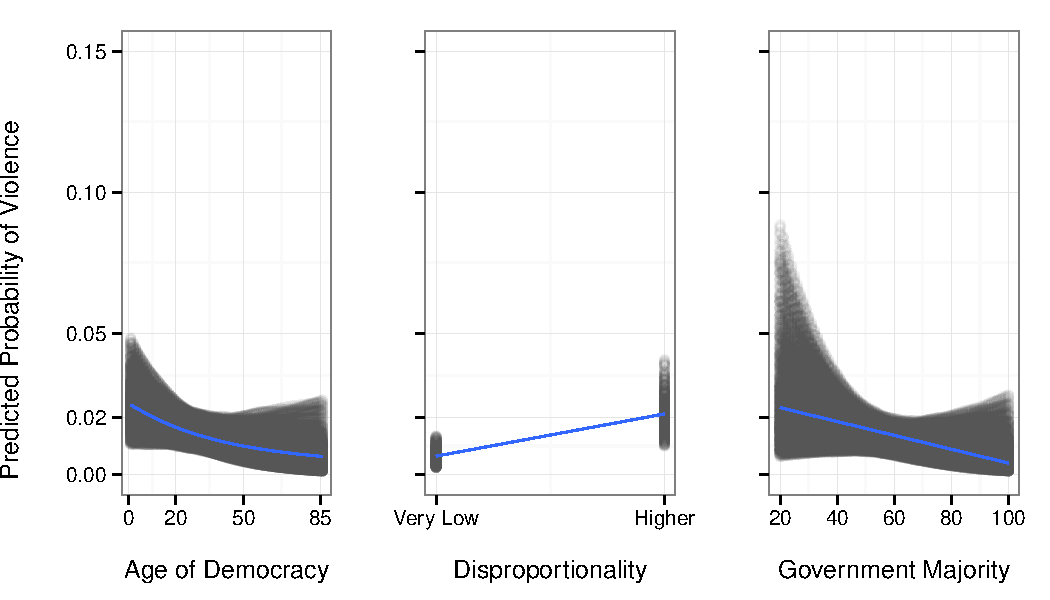
\includegraphics[width=0.8\linewidth]{figure/predProb} 

\end{knitrout}

    \end{center}
    \begin{singlespace}
      {\scriptsize{The graphs show the middle 95\% of 1000 simulations at each fitted value of the variables. The simulations use Model 15 with the sample constricted to observations from 1990. See Table \ref{outputTable.demNew}.}}
    \end{singlespace}
\end{figure}

%%%%%%%%%%%%%%%% Disproportionality Box Plot %%%%%%%%%%%%%%%%%%%%%%%%
\begin{figure}[t]
    \caption{Box Plots of Trust and Electoral Disproportionality When Legislative Violence is Observed and When it is Not. (Elected Legislatures)}  
    \label{BoxPlot}
    \begin{center}

\begin{knitrout}
\definecolor{shadecolor}{rgb}{0.969, 0.969, 0.969}\color{fgcolor}
\includegraphics[width=0.8\linewidth]{figure/boxplot} 

\end{knitrout}

    \end{center}
    \begin{singlespace}
        {\scriptsize{Note: values of the trust variable closer to 2 indicate less trust. Disproportionality is displayed using a logarithmic scale to ease interpretation. }}
    \end{singlespace}
\end{figure}

%%%%%%%%%%%%%%%% Scatterplot of Disproportionality, AgeDem, and Violence %%%%%%%%%%%%%%%%%%%%%%%%
\begin{figure}[t]
    \caption{Scatterplots of Disproportionality, Government Majority, Age of Democracy, and Violence in the Full Sample.}  
    \label{framework_empirical}
    \begin{center}

\begin{knitrout}
\definecolor{shadecolor}{rgb}{0.969, 0.969, 0.969}\color{fgcolor}
\includegraphics[width=0.8\linewidth]{figure/FrameworkEmpirical} 

\end{knitrout}

    \end{center}
    \begin{singlespace}
        {\scriptsize{From a sample of 200 countries between 1981 and 2008. The points are jittered horizontally.}}
    \end{singlespace}

\end{figure}

%%%%%%%% Variable source summary table
\begin{table}[!h]
    \begin{center}
    \caption{Base Variable Summary}
    \label{var_summary}
    \begin{tabular}{l m{7cm} m{3.5cm}}

            \hline
            Variable & Description & Source \\
            \hline \hline
            Disprop & Gallagher Index of Electoral Disproportionality & \cite{Gallagher2012} \& \cite{Carey2011} \\
            ENPS & Effective number of parties by seats & \cite{Gallagher2012} \& \cite{Carey2011} \\
            ENPV & Effective number of parties by votes & \cite{Gallagher2012} \& \cite{Carey2011} \\
            Ethnic Fractionalization & Probability two randomly selected members of society are from the same ethnic group & \cite{Alesina2003} \\
            Federal & Whether a country has a federal system or not & \cite{Carey2011}, updated from 2003 by the author \\           
            GDP/Capita & GDP per capita in thousands of US dollars & \cite{WorldBank2011} \\
            Gov. Fractionalization & Probability that two members of the Government will be from different parties & \cite{DPI2001} \\
            Gini & Gini Coefficient of income inequality & \cite{UNU2008} \\
            Immunity & Whether a legislators are immune from arrest and/or criminal prosecution or not & \cite{Fish2009} \\
            LEIC & Legislative Indices of Electoral Competition. Includes both the existence of a legislature and its electoral competitiveness. & \cite{DPI2001} \\
            Majority & Percentage of legislature controlled by governing parties & \cite{DPI2001} \\
            Polity & Polity IV Score & \cite{Marshall2009} \\
            PR & Whether a country uses a proportional representation electoral system or a plurality system & \cite{DPI2001} \\
            Self Expression & WVS self-expression indicator averaged across country-survey waves & \cite{WVS2009} \\
            System & Government system (parliamentary, presidential, or mixed & \cite{DPI2001} \\
            Tenshort & Tenure of the shortest serving veto player & \cite{DPI2001} \\
            Trust & Average of WVS responses where 1 $=$ most people can be trusted and 2 $=$ you can't be too careful & \cite{WVS2009} \\
            UDS & Posterior Mean Unified Democracy Score & \cite{Pemstein2010} \\
            Violence & Incidences of violence between legislators in the national parliamentary chamber & author \\
            \hline

    \end{tabular}
    \end{center}
    \begin{singlespace}
        Please contact the author for detailed summary statistics.
    \end{singlespace}
\end{table}  

%%%%%%%%%% Correlation matrix %%%%%%%%%% 
\begin{landscape}
\begin{figure}[t]
    \caption{Correlation Matrix for Variables Included in the Analysis (Elected Legislatures)}
    \label{corrmatrix}
    \begin{center}
    
    \includegraphics[width = \textwidth]{figure/corScatter.png}  
    %%% corScatter not created every compile to save time %%%
%<<corScatter>>=

%    library(corrgram)  

%    ### Create data set with variables for corrgram
%    vars.corrgram <- c("violence", "system", "DemAge", "maj", "MajCat", "govfrac", "singleParty", "pr", "tenshort", "UDS", "polity2", "ethnicAlesina", "CWtrust", "CWsurvSelfExpr", "disproportionality", "gini", "GDPperCapita", "enps", "enpv", "federal", "immunity")

%    # Subset elected legislature data
%    dem.corrData <- dem[vars.corrgram]

%    # Create corrgram
%    dem.corrgram <- corrgram(dem.corrData, order = TRUE, upper.panel = NULL, diag.panel = panel.minmax)

%@

    \end{center}
    \begin{singlespace}
        {\scriptsize{Redder squares indicate stronger negative bivariate correlations. \\
        Bluer squares indicate stronger positive bivariate correlations. \\
        Numbers in the diagonal squares indicate the minimum and maximum observed values of the variables in the sample.
        }}
    \end{singlespace} 
\end{figure}
\end{landscape}


%%%%%%%% Elected Legislatures Results Table
\begin{landscape}
\begin{table}
\caption{Legislative Violence Rare Events Logistic Regression Results (Elected Legislature)}
\label{outputTable.dem}
{\tiny{

\begin{tabular}{l c c c c c c c c c c c c c c c c }
\hline
                    & Model 1 & Model 2 & Model 3 & Model 4 & Model 5 & Model 6 & Model 7 & Model 8 & Model 9 & Model 10 & Model 11 & Model 12 & Model 13 & Model 14 & Model 15 & Model 16 \\
\hline
(Intercept)         & $-3.96^{***}$ & $-1.48^{***}$ & $-1.97^{***}$ & $-4.08^{***}$ & $-4.52^{***}$ & $-3.86^{***}$ & $-3.84^{***}$ & $-3.66^{***}$ & $-3.28^{***}$ & $-3.25$  & $-3.06^{***}$ & $-4.41$  & $-2.89$  & $-2.06^{**}$ & $-2.68^{*}$  & $2772678.51^{***}$  \\
                    & $(0.13)$      & $(0.37)$      & $(0.49)$      & $(0.18)$      & $(0.27)$      & $(0.35)$      & $(0.19)$      & $(0.27)$      & $(0.19)$      & $(4.90)$ & $(0.20)$      & $(4.21)$ & $(1.65)$ & $(0.78)$     & $(1.20)$     & $(1389.03)$         \\
DemAge              & $-0.01$       &               &               & $-0.01$       & $-0.01^{*}$   & $-0.02^{**}$  & $-0.01$       & $-0.02^{**}$  & $-0.02^{*}$   & $-0.01$  & $-0.01$       & $-0.02$  &          & $-0.02^{*}$  & $-0.02$      & $-0.03^{*}$         \\
                    & $(0.00)$      &               &               & $(0.00)$      & $(0.01)$      & $(0.01)$      & $(0.00)$      & $(0.01)$      & $(0.01)$      & $(0.01)$ & $(0.01)$      & $(0.01)$ &          & $(0.01)$     & $(0.01)$     & $(0.02)$            \\
maj                 &               & $-0.04^{***}$ & $-0.03^{***}$ &               &               &               &               &               &               &          &               &          &          & $-0.03^{**}$ & $-0.02$      & $0.01$              \\
                    &               & $(0.01)$      & $(0.01)$      &               &               &               &               &               &               &          &               &          &          & $(0.01)$     & $(0.01)$     & $(0.02)$            \\
UDS                 &               &               & $-0.24$       &               &               &               &               &               &               &          &               &          &          &              &              &                     \\
                    &               &               & $(0.18)$      &               &               &               &               &               &               &          &               &          &          &              &              &                     \\
immunity            &               &               &               & $0.27$        &               &               &               &               &               &          &               &          &          &              &              & $-0.94$             \\
                    &               &               &               & $(0.24)$      &               &               &               &               &               &          &               &          &          &              &              & $(0.73)$            \\
pr                  &               &               &               &               & $1.01^{***}$  &               &               &               &               &          &               &          &          & $0.76$       & $0.56$       & $0.01$              \\
                    &               &               &               &               & $(0.31)$      &               &               &               &               &          &               &          &          & $(0.49)$     & $(0.51)$     & $(0.93)$            \\
govfrac             &               &               &               &               &               & $-0.75$       &               &               &               &          &               &          &          &              &              & $-0.07$             \\
                    &               &               &               &               &               & $(0.67)$      &               &               &               &          &               &          &          &              &              & $(1.15)$            \\
enps                &               &               &               &               &               & $0.17$        &               &               &               &          &               &          &          &              &              & $-0.04$             \\
                    &               &               &               &               &               & $(0.09)$      &               &               &               &          &               &          &          &              &              & $(0.18)$            \\
singleParty         &               &               &               &               &               &               & $-0.19$       &               &               &          &               &          &          &              &              &                     \\
                    &               &               &               &               &               &               & $(0.24)$      &               &               &          &               &          &          &              &              &                     \\
disproportionality  &               &               &               &               &               &               &               & $0.01$        &               &          &               &          &          &              &              &                     \\
                    &               &               &               &               &               &               &               & $(0.02)$      &               &          &               &          &          &              &              &                     \\
HighProp            &               &               &               &               &               &               &               &               & $-1.24^{**}$  &          &               &          &          & $-1.39^{**}$ & $-1.26^{**}$ & $-2.39^{*}$         \\
                    &               &               &               &               &               &               &               &               & $(0.42)$      &          &               &          &          & $(0.43)$     & $(0.44)$     & $(1.10)$            \\
systemParliamentary &               &               &               &               &               &               &               &               &               & $0.31$   &               &          &          &              &              & $-2772667.75^{***}$ \\
                    &               &               &               &               &               &               &               &               &               & $(1.09)$ &               &          &          &              &              & $(1389.01)$         \\
systemPresidential  &               &               &               &               &               &               &               &               &               & $1.09$   &               &          &          &              &              & $-2772665.29^{***}$ \\
                    &               &               &               &               &               &               &               &               &               & $(1.05)$ &               &          &          &              &              & $(1389.01)$         \\
federal             &               &               &               &               &               &               &               &               &               & $-0.09$  &               &          &          &              &              & $0.59$              \\
                    &               &               &               &               &               &               &               &               &               & $(0.45)$ &               &          &          &              &              & $(0.67)$            \\
CWsurvSelfExpr      &               &               &               &               &               &               &               &               &               & $-0.74$  &               & $0.81$   &          &              &              & $0.21$              \\
                    &               &               &               &               &               &               &               &               &               & $(3.88)$ &               & $(3.47)$ &          &              &              & $(5.13)$            \\
tenshort            &               &               &               &               &               &               &               &               &               &          & $-0.23^{***}$ &          &          & $-0.07$      & $-0.10$      & $-0.02$             \\
                    &               &               &               &               &               &               &               &               &               &          & $(0.06)$      &          &          & $(0.08)$     & $(0.09)$     & $(0.15)$            \\
ethnicAlesina       &               &               &               &               &               &               &               &               &               &          &               & $-0.89$  &          &              &              & $3.19$              \\
                    &               &               &               &               &               &               &               &               &               &          &               & $(0.96)$ &          &              &              & $(1.80)$            \\
gini                &               &               &               &               &               &               &               &               &               &          &               & $0.00$   &          &              & $0.01$       & $-0.07$             \\
                    &               &               &               &               &               &               &               &               &               &          &               & $(0.02)$ &          &              & $(0.02)$     & $(0.05)$            \\
GDPperCapita        &               &               &               &               &               &               &               &               &               &          &               & $0.02$   &          &              & $0.01$       & $0.03$              \\
                    &               &               &               &               &               &               &               &               &               &          &               & $(0.02)$ &          &              & $(0.03)$     & $(0.03)$            \\
CWtrust             &               &               &               &               &               &               &               &               &               &          &               &          & $-0.66$  &              &              & $-7.56^{*}$         \\
                    &               &               &               &               &               &               &               &               &               &          &               &          & $(0.96)$ &              &              & $(3.69)$            \\
\hline
AIC                 & 710.94        & 656.15        & 551.50        & 708.06        & 647.35        & 416.41        & 690.17        & 421.44        & 409.68        & 232.46   & 674.73        & 292.50   & 390.76   & 388.37       & 358.25       & 165.47              \\
BIC                 & 723.36        & 668.66        & 569.43        & 726.62        & 665.31        & 438.07        & 708.66        & 438.00        & 426.23        & 259.37   & 693.32        & 321.29   & 400.87   & 421.31       & 401.45       & 240.25              \\
Log Likelihood      & -353.47       & -326.08       & -272.75       & -351.03       & -320.68       & -204.20       & -342.08       & -207.72       & -201.84       & -110.23  & -334.37       & -140.25  & -193.38  & -188.18      & -171.12      & -65.74              \\
\hline
\multicolumn{17}{l}{\scriptsize{\textsuperscript{***}$p<0.001$, 
  \textsuperscript{**}$p<0.01$, 
  \textsuperscript{*}$p<0.05$}}
\end{tabular}


}}
{\scriptsize{
	{*}{*}{*} $<$ 0.001 {*}{*} $<$ 0.01 {*} $<$ 0.05 {.} $<$ 0.1 \\
	Standard errors in parentheses. \\
	All models use robust (WEAVE) standard errors. \\
    Presidential is the reference category for government system variables (Assembly-Elected President and Parliamentary). \\
    Model 3 only includes observations where majority $<$ 90.
}}
\end{table}
\end{landscape}

%%%%%%%% Elected Legislatures (from 1990) Results Table
\begin{landscape}
\begin{table}
\caption{Legislative Violence Rare Events Logistic Regression Results (Elected Legislature, from 1990)}
\label{outputTable.demNew}
{\tiny{

\begin{tabular}{l c c c c c c c c c c c c c c c c }
\hline
                    & Model 1 & Model 2 & Model 3 & Model 4 & Model 5 & Model 6 & Model 7 & Model 8 & Model 9 & Model 10 & Model 11 & Model 12 & Model 13 & Model 14 & Model 15 & Model 16 \\
\hline
(Intercept)         & $-3.40^{***}$ & $-1.20^{**}$  & $-1.42^{**}$  & $-3.55^{***}$ & $-3.91^{***}$ & $-3.36^{***}$ & $-3.38^{***}$ & $-2.92^{***}$ & $-2.75^{***}$ & $-3.48$  & $-2.59^{***}$ & $-5.46$  & $-2.34$  & $-1.14$      & $-2.18$     & $3056797.29^{***}$  \\
                    & $(0.14)$      & $(0.40)$      & $(0.51)$      & $(0.20)$      & $(0.27)$      & $(0.37)$      & $(0.20)$      & $(0.30)$      & $(0.21)$      & $(5.05)$ & $(0.22)$      & $(4.41)$ & $(1.80)$ & $(0.81)$     & $(1.27)$    & $(1445.24)$         \\
DemAge              & $-0.01$       &               &               & $-0.01$       & $-0.02^{*}$   & $-0.02^{**}$  & $-0.01$       & $-0.03^{**}$  & $-0.02^{*}$   & $-0.01$  & $-0.01^{*}$   & $-0.03$  &          & $-0.02^{*}$  & $-0.03^{*}$ & $-0.02$             \\
                    & $(0.01)$      &               &               & $(0.01)$      & $(0.01)$      & $(0.01)$      & $(0.01)$      & $(0.01)$      & $(0.01)$      & $(0.01)$ & $(0.01)$      & $(0.02)$ &          & $(0.01)$     & $(0.02)$    & $(0.02)$            \\
maj                 &               & $-0.04^{***}$ & $-0.04^{***}$ &               &               &               &               &               &               &          &               &          &          & $-0.03^{**}$ & $-0.03^{*}$ & $0.00$              \\
                    &               & $(0.01)$      & $(0.01)$      &               &               &               &               &               &               &          &               &          &          & $(0.01)$     & $(0.01)$    & $(0.02)$            \\
UDS                 &               &               & $-0.25$       &               &               &               &               &               &               &          &               &          &          &              &             &                     \\
                    &               &               & $(0.20)$      &               &               &               &               &               &               &          &               &          &          &              &             &                     \\
immunity            &               &               &               & $0.31$        &               &               &               &               &               &          &               &          &          &              &             & $-0.34$             \\
                    &               &               &               & $(0.25)$      &               &               &               &               &               &          &               &          &          &              &             & $(0.78)$            \\
pr                  &               &               &               &               & $0.91^{**}$   &               &               &               &               &          &               &          &          & $0.45$       & $0.25$      & $0.21$              \\
                    &               &               &               &               & $(0.31)$      &               &               &               &               &          &               &          &          & $(0.50)$     & $(0.53)$    & $(0.96)$            \\
govfrac             &               &               &               &               &               & $-0.68$       &               &               &               &          &               &          &          &              &             & $-0.12$             \\
                    &               &               &               &               &               & $(0.71)$      &               &               &               &          &               &          &          &              &             & $(1.24)$            \\
enps                &               &               &               &               &               & $0.17$        &               &               &               &          &               &          &          &              &             & $0.01$              \\
                    &               &               &               &               &               & $(0.10)$      &               &               &               &          &               &          &          &              &             & $(0.19)$            \\
singleParty         &               &               &               &               &               &               & $-0.01$       &               &               &          &               &          &          &              &             &                     \\
                    &               &               &               &               &               &               & $(0.26)$      &               &               &          &               &          &          &              &             &                     \\
disproportionality  &               &               &               &               &               &               &               & $-0.01$       &               &          &               &          &          &              &             &                     \\
                    &               &               &               &               &               &               &               & $(0.02)$      &               &          &               &          &          &              &             &                     \\
HighProp            &               &               &               &               &               &               &               &               & $-1.13^{*}$   &          &               &          &          & $-1.19^{**}$ & $-1.16^{*}$ & $-1.99$             \\
                    &               &               &               &               &               &               &               &               & $(0.45)$      &          &               &          &          & $(0.46)$     & $(0.48)$    & $(1.10)$            \\
systemParliamentary &               &               &               &               &               &               &               &               &               & $-0.02$  &               &          &          &              &             & $-3056793.91^{***}$ \\
                    &               &               &               &               &               &               &               &               &               & $(1.15)$ &               &          &          &              &             & $(1445.22)$         \\
systemPresidential  &               &               &               &               &               &               &               &               &               & $1.40$   &               &          &          &              &             & $-3056791.15^{***}$ \\
                    &               &               &               &               &               &               &               &               &               & $(1.04)$ &               &          &          &              &             & $(1445.22)$         \\
federal             &               &               &               &               &               &               &               &               &               & $-0.48$  &               &          &          &              &             & $0.07$              \\
                    &               &               &               &               &               &               &               &               &               & $(0.53)$ &               &          &          &              &             & $(0.75)$            \\
CWsurvSelfExpr      &               &               &               &               &               &               &               &               &               & $-0.26$  &               & $2.05$   &          &              &             & $1.91$              \\
                    &               &               &               &               &               &               &               &               &               & $(4.00)$ &               & $(3.65)$ &          &              &             & $(5.58)$            \\
tenshort            &               &               &               &               &               &               &               &               &               &          & $-0.22^{***}$ &          &          & $-0.06$      & $-0.11$     & $0.01$              \\
                    &               &               &               &               &               &               &               &               &               &          & $(0.06)$      &          &          & $(0.08)$     & $(0.09)$    & $(0.16)$            \\
ethnicAlesina       &               &               &               &               &               &               &               &               &               &          &               & $-1.16$  &          &              &             & $3.09$              \\
                    &               &               &               &               &               &               &               &               &               &          &               & $(1.03)$ &          &              &             & $(2.13)$            \\
gini                &               &               &               &               &               &               &               &               &               &          &               & $0.00$   &          &              & $0.02$      & $-0.06$             \\
                    &               &               &               &               &               &               &               &               &               &          &               & $(0.02)$ &          &              & $(0.02)$    & $(0.05)$            \\
GDPperCapita        &               &               &               &               &               &               &               &               &               &          &               & $0.03$   &          &              & $0.04$      & $0.05$              \\
                    &               &               &               &               &               &               &               &               &               &          &               & $(0.02)$ &          &              & $(0.03)$    & $(0.04)$            \\
CWtrust             &               &               &               &               &               &               &               &               &               &          &               &          & $-0.68$  &              &             & $-4.86$             \\
                    &               &               &               &               &               &               &               &               &               &          &               &          & $(1.04)$ &              &             & $(4.25)$            \\
\hline
AIC                 & 601.46        & 561.44        & 462.68        & 598.70        & 561.14        & 346.04        & 583.29        & 348.10        & 339.58        & 189.18   & 574.10        & 241.91   & 326.53   & 322.26       & 296.09      & 133.28              \\
BIC                 & 613.20        & 573.26        & 479.83        & 616.24        & 578.38        & 366.64        & 600.77        & 363.85        & 355.33        & 214.48   & 591.65        & 269.09   & 336.03   & 353.58       & 337.21      & 203.17              \\
Log Likelihood      & -298.73       & -278.72       & -228.34       & -296.35       & -277.57       & -169.02       & -288.64       & -171.05       & -166.79       & -88.59   & -284.05       & -114.96  & -161.27  & -155.13      & -140.04     & -49.64              \\
\hline
\multicolumn{17}{l}{\scriptsize{\textsuperscript{***}$p<0.001$, 
  \textsuperscript{**}$p<0.01$, 
  \textsuperscript{*}$p<0.05$}}
\end{tabular}


}}
{\scriptsize{
	{*}{*}{*} $<$ 0.001 {*}{*} $<$ 0.01 {*} $<$ 0.05 {.} $<$ 0.1 \\
	Standard errors in parentheses. \\
	All models use robust (WEAVE) standard errors. \\
	Presidential is the reference category for government system variables (Assembly-Elected President and Parliamentary). \\
	Model 3 only includes observations where majority $<$ 90.
}}
\end{table}
\end{landscape}

%%%%%%%%%%%%%%%%%%%%%% Figures End %%%%%%%%%%%%%%%%%%%%%%%%%%%%%%%%%%%%%%%%%%%%%

\end{document}
